% CVPR 2027 submission. Template: CVPR 2026 author kit (https://github.com/cvpr-org/author-kit);
% swap cvpr.sty / ieeenat_fullname.bst for the 2027 kit when it is released.
\documentclass[10pt,twocolumn,letterpaper]{article}
\usepackage[review]{cvpr}
%% This file contains a number of tweaks that are typically applied to the main document.
%% They are not enabled by default, but can be enabled by uncommenting the relevant lines.


%%
%% Official support for 2-column teaser figure
%%
\usepackage{cuted} %< for strip environment

%%
%% For auto-referencing of figures (see fig/teaser.tex and \label{} therein) 
%%
\usepackage{currfile} %< for \currfilebase macro

%%
%% caption and (global) spacing overrides
%%
\usepackage{caption} %< for "\captionof" commands (teaser)
% \setlength{\abovecaptionskip}{.5em} % space above caption
% \setlength{\belowcaptionskip}{1em} % space below caption

%%
%% Inline annotations; for predefined colors, refer to "dvipsnames" in the xcolor package:
%% https://tinyurl.com/overleaf-colors
%%
\newcommand{\red}[1]{{\color{red}#1}}
\newcommand{\todo}[1]{{\color{red}#1}}
\newcommand{\TODO}[1]{\textbf{\color{red}[TODO: #1]}}
%%
%% Disable for camera ready / submission by uncommenting these lines:
%%
% \renewcommand{\TODO}[1]{}
% \renewcommand{\todo}[1]{#1}

%%
%% Work harder in optimizing text layout. Typically shrinks text by 1/6 of page, enable
%% it at the very end of the writing process, when you are just above the page limit.
%%
% \usepackage{microtype}

%%
%% Fine-tune paragraph spacing.
%%
% \renewcommand{\paragraph}[1]{\vspace{.5em}\noindent\textbf{#1.}}

%%
%% Globally adjusts space between figure and caption.
%%
% \setlength{\abovecaptionskip}{.5em}

%%
%% Allows "the use of \paper to refer to the project name"
%% with automatic management of space at the end of the word.
%%
% \usepackage{xspace}
% \newcommand{\paper}{ProjectName\xspace}

%%
%% Commonly used math definitions.
%%
% \DeclareMathOperator*{\argmin}{arg\,min}
% \DeclareMathOperator*{\argmax}{arg\,max}

%%
%% Tighten underline.
%%
% \usepackage{soul}
% \setuldepth{foobar}

%%
%% Reconfigure paragraph (tweaks spacing)
%%

%%
%% Project macros (Oct 17, 2026)
%%
\usepackage{booktabs}
\usepackage{array}
\newcommand{\RES}{\textbf{\color{red}[RES]}}                     % unmeasured number: never fill from memory
\newcommand{\CITE}[1]{\textbf{\color{red}[CITE: #1]}}            % citation not yet verified for the bib
\newcommand{\PLAN}[1]{{\color{orange}\textit{[Plan: #1]}}}        % outline text, replaced by prose

\definecolor{cvprblue}{rgb}{0.21,0.49,0.74}
\usepackage[pagebackref,breaklinks,colorlinks,allcolors=cvprblue]{hyperref}

\def\paperID{*****}
\def\confName{CVPR}
\def\confYear{2027}

\title{Simulate Only What Matters:\\Certified Sparse Simulator Probing for Physics-Grounded Video Generation}
\author{Anonymous}

\begin{document}
\twocolumn[{%
\renewcommand\twocolumn[1][]{#1}%
\maketitle
\begin{center}
\centering
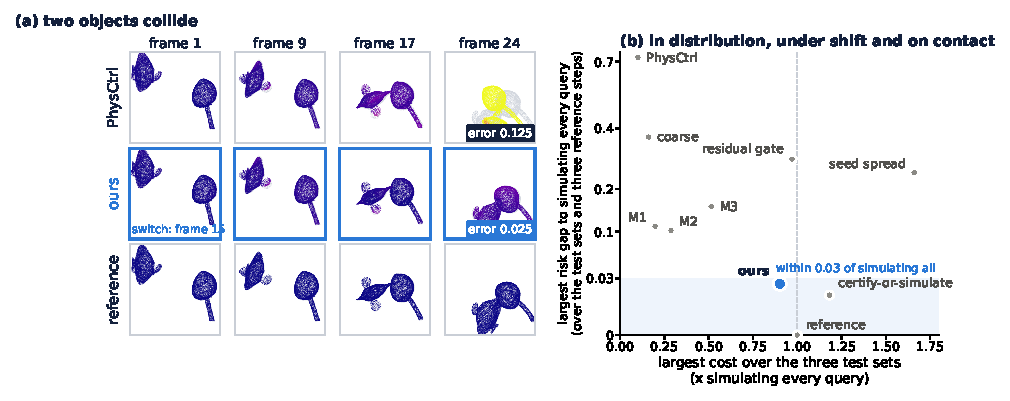
\includegraphics[width=\linewidth]{fig/teaser.pdf}
\captionof{figure}{\textbf{A fast motion prior fails silently; a few simulator checks catch it.}
(a) Two objects collide (the median rejected test scene with a mid-clip switch, chosen before any picture; colour is each point's distance to the reference simulation). PhysCtrl moves each object as if it were alone and misses the collision; ours detects the approach, switches to a contact-resolving simulation at frame 15 and follows the reference.
(b) Every pipeline of \cref{tab:main} over the in-distribution, shifted and two-object test sets: largest risk gap to simulating every query (over the sets and three reference time steps, \cref{sec:res-reference}) against largest cost: ours is the only one within 3 points at less than that cost.}
\label{fig:teaser}
\end{center}%
}]
\begin{abstract}
Physics-grounded video generators move objects along a 3D trajectory predicted by a learned motion prior.
On familiar queries such a prior can rival a physics simulator, but nothing tells the user when a query is not familiar: on our tests, PhysCtrl's trajectories are wrong for 68\% of queries outside its training range and for 69\% of two-object collisions, and its own uncertainty does not flag them.
We generate each trajectory once and then check it with a few short runs of the simulator it was trained to imitate.
A calibrated threshold turns the check into an accept-or-reject certificate that bounds how many bad trajectories are accepted.
A rejected trajectory keeps the part that passed; only the rest is re-simulated, and before a collision a cheap simulation decides when to switch to a contact-resolving setting.
In pre-registered tests on fresh data, re-scored against the simulator at three time steps, PhysCtrl's failures persist whichever step is taken as ground truth, while ours stays within 2.5 points of the risk of simulating every query, in distribution, under four kinds of shift and on contact, at 0.26$\times$, 0.71$\times$ and 0.90$\times$ its cost.
Tuned cheaper simulator settings win where the regime is known in advance, but each is ten or more points riskier than the full simulator on some test set.
% src: Phase 9 (results/p9_table); Phase 10c T1 (pre-registered) and max gap (exploratory, results/p10c_explore); 4m
\end{abstract}

\section{Introduction}
\label{sec:intro}

Physics-grounded video generation separates motion from appearance: a model predicts how the points of an object move under the requested forces, and a video model renders that trajectory~\cite{wang2025physctrl}.
The motion model is a learned prior, fast enough to sample in a fraction of a second, and on its own examples its videos are judged on par with those driven by a physics simulator~\cite{wang2025physctrl}.
But a query need not be familiar.
On our tests, PhysCtrl's trajectory model is wrong for 68\% of queries whose material or forces lie outside its training range and for 69\% of scenes in which two objects collide (\cref{fig:teaser}a).
% src: Phase 9 (generate only: shift 0.680, contact 0.693)
These failures are silent: a rendered clip can look plausible while its physics is wrong~\cite{khanbayov2026physweep}, and the model's own uncertainty, the spread between its samples, accepted 99\% of the failed drops in our shift test.
% src: Phase 4m (seed spread accepts 99% of drop failures)

The obvious remedies each give something up.
Simulating every query with the physics engine that produced the training data~\cite{foo2026physical, liu2026realwonder} matches that data by construction but costs about twenty generations per query.
% src: Phase 1 (reference 4.666 s vs generation 0.236 s, A100)
A cheaper simulator setting, tuned as a fair efficiency comparison requires~\cite{mcgreivy2024weak}, is excellent in distribution (1.5\% wrong at 13\% of the cost), yet under shift the same setting is wrong about 10 points more often than the full simulator, whichever time step of the simulator is taken as ground truth.
% src: Phase 9 (always M1: 0.015 / 0.13x ID); Phase 10c T3 for M1 (gap +0.10 to +0.11 against dt, dt/2, dt/4)
Since a user cannot tell in advance which queries are unfamiliar, we ask: \emph{can each generated trajectory be trusted or corrected per query, at less than the cost of simulating it?}

We answer by generating the trajectory once and spending the simulator only where it is needed (\cref{fig:method}).
A few short simulator runs, restarted from states read off the generated frames, measure how far the trajectory drifts from physics; no equation residual is needed.
A threshold calibrated on separate objects turns this drift into a certificate that bounds the fraction of bad trajectories it accepts.
A rejected trajectory keeps its certified prefix, and only the rest is re-simulated, starting from the full state of a cheap shadow simulation of the true initial state.
Before a collision, where cheap grids fail, the same shadow decides when to hand over to a setting that resolves the contact.
\Cref{fig:teaser}b summarises the outcome: across the three test sets and against three time steps of the reference, ours is the only pipeline that stays within 3 points of the risk of simulating every query while costing less.
% src: Phase 10c (max gap, exploratory)

Our contributions are:
\begin{itemize}
\item \textbf{A certificate for generated motion}: a few short simulator checks, calibrated at the object level so that the fraction of bad trajectories accepted is bounded in distribution; under shift it accepted 1.2\% of failures, against 35\% for the generator's own uncertainty.
% src: Phase 4a extension (0.084 <= 0.11); Phase 4m M1 (0.012 vs 0.353)
\item \textbf{Repair that re-simulates only what failed}, from a cheap shadow's state, with \textbf{event-aware fidelity}: the shadow times the switch to a contact-resolving setting, which halves the repaired error on collisions. Repairing with the generator itself does not work (five attempts, at most 1\% better).
% src: Phase 9 CC3 (0.029 -> 0.015); Phases 4b-4g-v2
\item \textbf{A pre-registered, compute-accounted evaluation} on new shift and two-object contact benchmarks, against tuned simulators and gating baselines, and re-scored against the reference at three time steps: ours tracks the full simulator everywhere at 0.26--0.90$\times$ its cost; tuned settings are cheaper where the regime is known, and one of them (M2) matches ours under shift once the simulator's own time-step uncertainty is taken into account.
% src: Phase 9; Phase 10c (T1 PASS, T3 PASS for M1/M3, FAIL for M2; max gap exploratory)
\end{itemize}

We study elastic objects with PhysCtrl's base model. Where the regime of a query is known in advance, a tuned simulator is cheaper than our pipeline; we report this throughout: ours pays for not knowing.

\section{Related work}
\label{sec:related}

\paragraph{Physics-grounded video generation.}
One line of work drives video synthesis with explicit physics.
PhysCtrl~\cite{wang2025physctrl} generates 3D point trajectories with a diffusion model trained on simulated data and renders them, which is fast but inherits the generator's errors.
PSIVG~\cite{foo2026physical} and RealWonder~\cite{liu2026realwonder} instead run a physical simulator for the clip and condition the video on its output, PhysMAS~\cite{qin2026physmas} assigns part-wise materials with agents and simulates every multi-object scene in a shared MPM domain, and PhysStream~\cite{chen2026physstream} adds structured scene memory for streaming control.
NEXUS~\cite{ying2026nexus} learns contact-rich object dynamics from energy and dissipation fields, a better prior for the collisions on which PhysCtrl fails; a certificate like ours could check such a prior as well.
These methods either trust a learned prior or simulate every query in full; we generate once and spend the simulator only on short windows and uncertified suffixes.

\paragraph{Evaluating physics in generated video.}
Physics-IQ~\cite{motamed2025do} and VideoPhy-2~\cite{bansal2025videophy} test whether generated videos respect physical principles and commonsense, RigidBench~\cite{jain2026rigidbench} compares generated motion with a simulator rollout from the same initial state, and PhysWeep~\cite{khanbayov2026physweep} shows that a clip can look plausible while encoding the wrong value of the governing physical parameter.
We follow the simulator-grounded view: we score 3D trajectories against the reference simulator, since plausibility alone does not reveal a wrong trajectory (\cref{sec:results}).

\paragraph{Trusting learned surrogates.}
Hybrid neural world models~\cite{lakshmanan2026hybrid} note that neural surrogates fail silently at shocks, fronts and contact, and use a per-trajectory error map to gate a fallback to a reference solver; ANCHOR~\cite{roy2025anchor} triggers classical-solver corrections of a neural-operator rollout when a residual-based error estimate grows; HyPER~\cite{srikishan2025model} learns a cost-aware policy for calling the simulator; NeuroForge~\cite{jabbary2026neuroforge} audits a CFD surrogate with its physics residual and finds the residual a reliable trust signal rather than a correction objective, in line with our negative repair results; and threshold-aware conformal routing~\cite{tan2026threshold} decides per input whether a surrogate's scalar output can be used.
These methods gate a deterministic surrogate on a signal computed from the surrogate itself.
We gate a stochastic generative model of a whole trajectory with reference-simulator probes restarted from lifted states, need no residual, and certify the accepted set with a finite-sample guarantee; we also compare against a residual-based gate directly (\cref{sec:results}).

\paragraph{Conformal and selective prediction.}
Split conformal prediction~\cite{angelopoulos2021gentle} gives distribution-free guarantees under exchangeability; hierarchical variants~\cite{dunn2023distribution} handle correlated groups, which motivates our object-level calibration.
Conformal methods have been applied to neural PDE surrogates~\cite{gopakumar2024uncertainty, gopakumar2025calibrated}, to multi-tier model cascades~\cite{dou2026conformal}, and to distribution shift through adaptive recalibration~\cite{gibbs2021adaptive}, which our amortised verifier would need under drifting query streams.

\paragraph{Coarse--fine coupling and constrained sampling.}
Our repair resembles one step of Parareal-style coupling, where a cheap solver supplies states that a fine solver corrects~\cite{pamela2025neural}; it differs in being a single verification-gated restart rather than an iteration to convergence, with a learned generative prior as the predictor.
Inference-time constraints for generative models~\cite{cohan2024flexible, utkarsh2025physics} could in principle repair a trajectory from its verified frames; for PhysCtrl, the five generative repairs we tried (three training-free, two fine-tuned) improved the error by at most 1\%, and we explain why in \cref{sec:repair}.

\section{Method}
\label{sec:method}
\begin{figure*}[t]
\centering
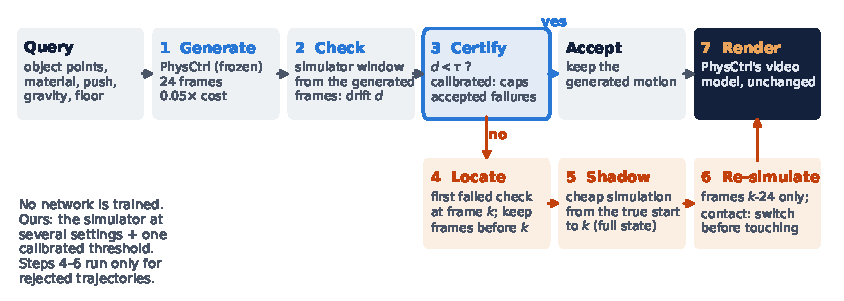
\includegraphics[width=\linewidth]{fig/method.pdf}
\caption{\textbf{Generate once, simulate only what fails.} A generated trajectory is checked by short simulator windows restarted from its own frames (\cref{sec:probes}) and certified by a calibrated threshold (\cref{sec:certificate}). A rejected trajectory keeps its certified prefix; only the rest is re-simulated, from a cheap shadow simulation of the true start (\cref{sec:repair}), and at contacts the shadow times the switch to a contact-resolving setting (\cref{sec:fidelity}).}
\label{fig:method}
\end{figure*}

\subsection{Problem and risk}
\label{sec:problem}
A query $q = (\mathbf{x}_0, \theta)$ consists of an object's initial particle positions $\mathbf{x}_0 \in \mathbb{R}^{N\times 3}$ and physical parameters $\theta$ (Young's modulus $E$, Poisson ratio $\nu$, drag forces, gravity, floor).
A generator $G$ (PhysCtrl's trajectory diffusion model~\cite{wang2025physctrl}) returns a trajectory $\hat{\mathbf{x}}_{1:T} = G(q)$ of $T = 24$ frames.
The reference simulator $S$ is the Material Point Method (MPM)~\cite{jiang2016material} solver that produced the generator's training data, run at its own setting; its rollout $\mathbf{x}_{1:T} = S(q)$ is the ground truth.
This is the motion the generator was trained to imitate, not real-world motion; we test its numerical convergence in \cref{sec:res-reference}.
% src: Phase 0 (replay error ~2e-6; same simulator for data and probes)
The error of a trajectory is the mean point distance $e(\hat{\mathbf{x}}) = \frac{1}{TN}\sum_{t,i} \lVert \hat{\mathbf{x}}_{t,i} - \mathbf{x}_{t,i} \rVert$, and a trajectory is \emph{bad} if $e > \varepsilon$.
We use $\varepsilon = 0.10$, about 5\% of the object size.
The \emph{risk} of a pipeline is the probability that its output is bad; its \emph{cost} is the compute it spends per query, relative to always running $S$.

\subsection{Sparse window probes}
\label{sec:probes}
A probe checks whether a short stretch of $\hat{\mathbf{x}}$ is consistent with physics.
At model frame $k$ we lift a simulator state $z_k$ from the generated frames: positions are read directly, velocities come from a three-point quadratic finite difference in time, the affine velocity field from a local least-squares fit over 12 neighbours, and the deformation gradient is set to the identity.
Lifting the deformation gradient from noisy generated positions made the simulator unstable even on ground-truth trajectories, while the identity never did.
% src: Phase 2 v1 NO-GO (F-lift blow-ups) vs Phase 2-v2 (lift_noF, 0 blow-ups)
We run a cheap simulator $S_c$ from $z_k$ for $m$ frames and measure the drift
\begin{equation}
  d_k = \tfrac{1}{N}\textstyle\sum_i \lVert S_c(z_k)_{k+m,i} - \hat{\mathbf{x}}_{k+m,i} \rVert .
\end{equation}
The defect needs no residual of the governing equations, only the simulator.
$S_c$ is the same MPM solver on a $64^3$ grid with a time step set by the CFL condition, $\Delta t = \min(8{\times}10^{-4}, 0.5\,\Delta x / c)$ for wave speed $c$; it keeps the signal of the reference setting at one eighth of the cost.
% src: Phase 2c verdict A' PASS
We use $m = 4$ frames.
For a single object, one window suffices: it starts at the strongest event in the generated motion (peak acceleration or floor proximity).
Two further windows spread over the remaining start frames rank errors no better (AUROC 0.958 vs.\ 0.955 on development data) at three times the probe cost.
% src: pilot E2 (exploratory, development data); placement spread_event chosen on Phase 2c by a pre-stated rule
For two-object scenes we keep all three windows: a generation that ignores a collision has no event at the collision, so the event window alone misses it.
% src: Phase 9 amendment before data (code check on seen 4o scenes: one window -> SF risk 0.095)
A window whose rollout blows up scores $d_k = +\infty$, an automatic reject.
% src: pre-registered Oct 10 (blow-up rule)
The certificate score is $s(\hat{\mathbf{x}}) = \max_k d_k$ over the placed windows.

\subsection{Object-level conformal certificate}
\label{sec:certificate}
We accept $\hat{\mathbf{x}}$ if $s(\hat{\mathbf{x}}) < \tau$ and calibrate $\tau$ on bad trajectories only.
Calibration queries come from objects that never appear at test time, several physical draws per object.
Because draws of one object are correlated, we calibrate at the object level: from each calibration object with at least one bad draw we pick one bad draw uniformly at random, and set $\tau$ to the $\lfloor \alpha (n+1) \rfloor$-th smallest of these $n$ scores.
For a new object exchangeable with the calibration objects, split conformal prediction then gives
\begin{equation}
  P\big(s(\hat{\mathbf{x}}) < \tau \,\big|\, e(\hat{\mathbf{x}}) > \varepsilon\big) \le \alpha ,
\end{equation}
so the risk of an accepted output is at most $\alpha\,P(e > \varepsilon)$.
With $\alpha = 0.10$ we obtain $\tau = 0.02614$ for the three-window score.
% src: Phase 4a extension (object-level), replicate 0; validity 0.084 <= 0.11 over 500 splits
The same calibration gives the one-window score a threshold of 0.0301; accepting a single window below the smaller $\tau$ accepts a subset of what that rule accepts, so the bound carries over.
% src: pilot E2 (variant a, threshold 0.03007); Phase 9 uses tau = 0.02614 for both
The guarantee holds in distribution. Under shift it is not guaranteed, and we test it empirically (\cref{sec:results}).

\subsection{Repairing only the uncertified suffix}
\label{sec:repair}
A rejected trajectory could be regenerated with its verified frames fixed.
We tried five such generative repairs, three training-free and two fine-tuned; the best improved the error by 1\% (\cref{sec:results}). A restart from generated states removes only 20\% of the error at its own frames, against 94\% from the true initial state, so verification does not supply correction; and optimising the generation against the defect lowered the defect while the true error doubled.
% src: Phase 4g-v2 diagnosis (20% vs 94%); Phase 4c (0.267 -> 0.511)
We therefore repair by simulation, and only where needed.

On rejection we walk a chain of windows: an anchor window from the true initial state, then windows starting at model frames $k \in \{3, 7, 11, 15, 19\}$, reusing windows the certificate already ran.
If the first failing window starts at frame $k$, we keep the generated frames up to $k$ and re-simulate the rest.
If the anchor fails, or no chain window fails, the whole trajectory is simulated with the reference setting.
The restart needs a full simulator state (positions, velocities, deformation gradients, affine velocities), which the generated frames cannot provide.
A \emph{shadow} supplies it: a cheap simulation from the true initial state up to frame $k$, whose full state starts the suffix.
% src: Phase 4h (restart from generated positions: risk 0.070) -> 4i V2 (shadow state: risk 0.017) -> 4k confirmation
The shadow is cheap and starts from the truth, so it carries the stress state that a restart from generated positions loses.

The suffix only has to meet the error target, not to reproduce the reference exactly.
We therefore run the shadow and the suffix at tuned settings of the same MPM solver:
the shadow at $\mathrm{M1}$ ($96^3$ grid, $\Delta t \le 8{\times}10^{-4}$) and the suffix at $\mathrm{M2}$ ($96^3$ grid, $\Delta t \le 4{\times}10^{-4}$), both capped at CFL number 0.5.
On development data this medium-fidelity suffix cut the cost of our pipeline by 25--55\% at similar risk.
% src: pilot 8a (exploratory, B2); Phase 9 confirmation uses M1 shadow + M2 suffix

\subsection{Event-aware fidelity at contact}
\label{sec:fidelity}
When two objects collide, the coarse grid cannot resolve the gap between them, so both the coarse check and the coarse shadow become unreliable near contact.
% src: Phase 4l diagnosis (dx 0.156 vs contact gap 0.16); 4l-ref H0 PASS at the reference setting
Instead of placing more windows at the contact, which did not help, we switch fidelity before it.
% src: Phase 4l H1-H3 FAIL
A coarse shadow from the true initial state records the distance between the two objects; at the first frame $k_{\mathrm{sh}}$ where they come within three coarse cells ($0.47$ units), a contact-resolving setting takes over from frame $\max(k_{\mathrm{sh}}-1, 1)$, restarted from the shadow's state.
This setting, $\mathrm{M3}$, uses the reference solver's $125^3$ grid with $\Delta t \le 2{\times}10^{-4}$; it was the cheapest setting within the error target on the development contact scenes.
% src: pilot 8a (M3 risk 0.004 on 4l contact scenes; M2 0.031); Phase 9 contact pipeline
If the shadow's objects start that close or never come that close, the scene is simulated with the reference setting.
Timing the switch from the generation instead, whose contact is itself wrong, narrowly missed its risk margin.
% src: Phase 4n N1 FAIL (0.034 vs 0.030); Phase 4o CONFIRMED

\subsection{Cost accounting}
\label{sec:cost}
All costs are A100 seconds per query: one generation costs 0.236\,s and one reference rollout 4.666\,s.
Probe windows are charged by a linear fit in simulator substeps, the shadow and the suffix by their substeps relative to a full reference rollout (the coarse shadow by its measured rate).
At 2{,}048 particles a substep costs almost the same on every grid we use (A100: 0.229\,ms at $64^3$, 0.233\,ms at $125^3$; H200: 0.29--0.32\,ms from $64^3$ to $125^3$), so charging simulator work by substeps treats all settings alike.
% src: p4d_fullsim coarse rate vs c_ref/20016 (A100); p9_full / p9c_full rollout_s per substep (H200), checked Oct 19
% src: Phase 1 timings; 4k cost model

\section{Experimental setup}
\label{sec:setup}

\paragraph{Generator and simulator.}
We use PhysCtrl's base trajectory model~\cite{wang2025physctrl} (2{,}048 points, 24 frames, 4 sampling steps) and its MPM simulator at PhysCtrl's own setting as the reference, so that ground truth and probes come from the same simulator.
% src: Phase 0 (replay ~2e-6; matches PhysCtrl eval.py within 3%)

\paragraph{Benchmarks.}
All queries are elastic objects from PhysCtrl's released test set with physical parameters drawn by us; ground truth is the reference rollout.
\begin{itemize}
\item \emph{Calibration pool}: 1{,}200 queries (12 in-distribution draws of $E$, $\nu$ and the drag force for each of 100 objects), used only to set thresholds.
% src: id_new_0..11
\item \emph{In distribution}: 200 fresh draws on the same objects, two per object.
% src: Phase 9 (id_new_22, id_new_23)
\item \emph{Shift}: 400 fresh queries in four families of 100, each moving one parameter outside the training range: softer ($E \in 10^{[3.0, 3.9]}$\,Pa), stiffer ($10^{[7.1, 7.8]}$\,Pa), stronger drag, and a drop under gravity onto a floor 0.1--0.5 below the object, which PhysCtrl's elastic training data never contains.
% src: Phase 9 (ood3_*: the 4m ood2 distributions, new draws)
\item \emph{Two-object contact}: 132 scenes in which two objects collide, plus 36 control scenes in which they stay apart; PhysCtrl generates each object separately and the outputs are composed, the ground truth is a joint simulation.
A pre-registered sanity rule on the joint simulation excluded 32 of 200 designed scenes.
% src: Phase 9 contact (draws 24-27)
\item \emph{Development sets} for the analyses and ablations, each also fresh when its own test ran: 800 in-distribution queries (4k), 398 shifted queries (4m), and 346 contact scenes (4o).
\item \emph{Videos}: PhysCtrl's five elastic image examples, as given and with 3$\times$ the drag force, rendered with PhysCtrl's own pipeline.
% src: 6a
\end{itemize}

\paragraph{Protocol.}
Every test was pre-registered, with its decision rule and margin, before its data existed; thresholds were never refit on test data; negative outcomes are reported.
The final configuration and its seven tests were fixed before the in-distribution, shift and contact test sets above were generated. One amendment, also made before the data, kept three windows for contact scenes and added absolute risk bounds to the relative tests.
% src: PLAN.md Phase 9 pre-registration and amendment (Oct 19)
Uncertainty is an object-cluster bootstrap (2{,}000 resamples), since draws of one object are correlated.
Risk and mean error weight each object equally.

\paragraph{Baselines.}
\emph{Generate only} (PhysCtrl);
\emph{coarse only} (the cheap simulator alone);
\emph{always simulate at a tuned setting} $\mathrm{M1}$, $\mathrm{M2}$ or $\mathrm{M3}$ (\cref{sec:repair,sec:fidelity}), the cheapest settings of the reference solver that met the error target on development data; a learned or cheap method should be compared against a tuned solver, not only the default one~\cite{mcgreivy2024weak};
\emph{seed-spread deferral} (8 samples, simulate if their spread exceeds a threshold calibrated like ours);
\emph{accept coarse if it agrees} (run the cheap simulator, accept it when it agrees with the generation, else simulate with the reference setting);
\emph{momentum-residual gate} (accept the generation when its centre of mass follows momentum balance, in the spirit of residual-triggered correction~\cite{roy2025anchor});
\emph{best-of-8} (select one of 8 samples by medoid or by residual);
\emph{certify or simulate} (our certificate, with a full reference rollout on rejection);
\emph{always simulate}.
Ablations: uniform window placement at matched budget, shuffled restart times, and a switch timed by the generation instead of the shadow.

\paragraph{Metrics.}
Risk ($P(e > 0.10)$, also at 0.05 and 0.20), mean, tail and last-frame error, the certificate's false-accept rate on bad trajectories, AUROC and the area under the risk--coverage curve (AURC) of each score, and cost relative to always simulating.
On PhysCtrl's test set we also report PhysCtrl's own metrics, position MSE and its deformation loss.

\section{Results}
\label{sec:results}

\begin{table*}[t]
\centering
\small
\setlength{\tabcolsep}{4.2pt}
% generated by code/p9_table.py from the Phase 9 rows (contact cells marked \dagger: Phase 7d); do not edit by hand
\begin{tabular}{@{}lcccccccc@{}}
\toprule
 & \multicolumn{2}{c}{In distribution} & \multicolumn{2}{c}{Shift} & \multicolumn{2}{c}{Two-object contact} & \multicolumn{2}{c}{All three} \\
\cmidrule(lr){2-3}\cmidrule(lr){4-5}\cmidrule(lr){6-7}\cmidrule(l){8-9}
Pipeline & risk & cost & risk & cost & risk & cost & max gap & max cost \\
\midrule
\multicolumn{9}{@{}l}{\textit{Learned prior}} \\
PhysCtrl & \textcolor{gray}{0.130} & 0.05 & \textcolor{gray}{0.680} & 0.05 & \textcolor{gray}{0.693} & 0.10 & \textcolor{gray}{$+$0.722} & 0.10 \\
\multicolumn{9}{@{}l}{\textit{Fixed simulator setting}} \\
Coarse & \textcolor{gray}{0.040} & 0.13 & \textcolor{gray}{0.367} & 0.16 & \textcolor{gray}{0.318$^\dagger$} & 0.12$^\dagger$ & \textcolor{gray}{$+$0.367$^\dagger$} & 0.16$^\dagger$ \\
Tuned M1 & \textbf{0.015} & \textbf{0.13} & \textcolor{gray}{0.102} & 0.20 & \textbf{0.029} & \textbf{0.13} & \textcolor{gray}{$+$0.111} & 0.20 \\
Tuned M2 & 0.020 & 0.25 & \textcolor{gray}{0.102} & 0.29 & \textcolor{gray}{0.035} & 0.25 & \textcolor{gray}{$+$0.102} & 0.29 \\
Tuned M3 & 0.015 & 0.50 & \textcolor{gray}{0.155} & 0.51 & 0.000 & 0.50 & \textcolor{gray}{$+$0.155} & 0.51 \\
Reference (simulate all) & 0.000 & 1.00 & 0.000 & 1.00 & 0.000 & 1.00 & $+$0.000 & 1.00 \\
\multicolumn{9}{@{}l}{\textit{Gated}} \\
Seed-spread deferral & 0.000 & 1.11 & \textcolor{gray}{0.247} & 1.06 & \textcolor{gray}{0.086$^\dagger$} & 1.66$^\dagger$ & \textcolor{gray}{$+$0.247$^\dagger$} & 1.66$^\dagger$ \\
Momentum residual & 0.010 & 0.77 & 0.007 & 0.97 & \textcolor{gray}{0.290$^\dagger$} & 0.69$^\dagger$ & \textcolor{gray}{$+$0.290$^\dagger$} & 0.97$^\dagger$ \\
Certify or simulate & 0.015 & 0.54 & 0.003 & 0.87 & 0.000 & 1.18 & $+$0.015 & 1.18 \\
\midrule
\textbf{Ours} & 0.020 & 0.26 & \textbf{0.013} & \textbf{0.71} & 0.012 & 0.90 & \textbf{$+$0.025} & \textbf{0.90} \\
\bottomrule
\end{tabular}

\caption{\textbf{Every pipeline on the three test sets.}
Risk is the fraction of outputs with error above $\varepsilon = 0.10$; cost is compute per query relative to simulating it with the reference. Each object counts once.
Risks are against the reference at PhysCtrl's time step $\Delta t$, as pre-registered; \cref{tab:reference} repeats them against $\Delta t/2$ and $\Delta t/4$.
\emph{All three}: the largest gap to simulating every query, risk(pipeline) $-$ risk(reference at $\Delta t$), over the three sets and the three reference steps (defined after the Phase 10c verdict), and the largest cost.
Grey: risk above 0.03, or a gap above 0.03. Bold: the cheapest pipeline within 0.03 in each column.
M1--M3 are the reference solver at tuned cheaper settings. $^\dagger$: not run on this contact set; value from an earlier contact set (\cref{sec:res-contact}).}
\label{tab:main}
% src: results/p9_table (generated by code/p9_table.py from the Phase 9 rows; dagger cells from results/p7d_contact)
\end{table*}

\subsection{Main comparison}
\label{sec:res-main}
\Cref{tab:main} and \cref{fig:teaser}b compare all pipelines on the final test sets, each generated after the pipeline and its seven tests were fixed; all seven tests pass.
% src: Phase 9 (pre-registered Oct 19; verdicts results/p9_confirm, results/p9c_summary)

\paragraph{Ours tracks the simulator it replaces.}
Against the pre-registered reference, ours has risk 0.013 under shift at 0.71$\times$, saving 0.76\,s per query against certify-or-simulate (99\% CI [0.62, 0.91]) and 0.090 [0.055, 0.128] less risky than M1.
% src: Phase 9 C4, C5 (99% CIs, Bonferroni over five)
Re-scored against references at half and a quarter of the time step (\cref{sec:res-reference}), ours stays within 2.5 points of the risk of simulating every query on every set, the only pipeline below the simulator's cost to do so (\cref{tab:main}).
Each fixed setting is at least ten points riskier than the full simulator on some set: M1 and M3 under shift against every reference, coarse under shift, and M2 under shift against $\Delta t$; PhysCtrl fails everywhere outside its training regime.
The two other pipelines within the gap cost more than simulating on contact (certify-or-simulate 1.18$\times$) or are the simulator itself.
% src: Phase 10c (T3 for M1/M3, pre-registered; max gap, exploratory: results/p10c_explore)
The saving comes from the milder shifts: on the softer and stiffer families ours costs 0.50$\times$ and 0.24$\times$, while on 3$\times$ drag and drops almost every generation is rejected and ours costs as much as simulating (0.99$\times$, 1.10$\times$), as it should.
% src: Phase 9 per family (p9_confirm.assemble, Oct 20)

\paragraph{In distribution, safety has a price.}
Ours has risk 0.020 at 0.26$\times$ (99\% CI [0.21, 0.31]$\times$), 1.30\,s per query cheaper than certify-or-simulate ([1.03, 1.55]).
A tuned simulator is cheaper still (M1: 0.015 at 0.13$\times$), as we stated before the test; it stays safe only while the query resembles the data it was tuned on.
% src: Phase 9 C1-C3; pre-registration ("reported either way")

\subsection{The certificate}
\label{sec:res-cert}
On the final test sets the certificate accepted 1 of 272 bad generations under shift, 3 of 26 in distribution and 0 of 87 on contact; it is conservative, accepting 105 of 174 good generations in distribution and 1 of 45 on contact.
% src: results/p9_table (descriptive)
On the calibration objects the object-level guarantee held (false-accept rate 0.084, within the finite-sample bound of 0.11).
Under shift the window certificate let through 1.2\% of failures, whereas PhysCtrl's own uncertainty, the spread of eight samples, let through 35\% and accepted 99\% of the failed drops.
As a ranker of generation error (risk--coverage curves in the supplement) the window score has AUROC 0.977, against 0.886 for the momentum residual and 0.671 for seed spread, which is worse than random acceptance at low coverage; only a full coarse rollout ranks as well (0.973), at the cost of the rollout. The best of eight samples cannot fix shift: even the oracle choice is wrong for 68\% of shifted queries.
% src: Phase 4a extension (500 splits); 4m M1 (0.012; +0.341); 7a Q1, Q4 (development pool)

\subsection{Ablations}
\label{sec:res-ablation}
\begin{table}[t]
\centering
\footnotesize
\setlength{\tabcolsep}{3pt}
\begin{tabular}{@{}>{\raggedright\arraybackslash}p{3.55cm}>{\raggedright\arraybackslash}p{2.75cm}l@{}}
\toprule
Change & Effect & Source \\
\midrule
Restart the repair from generated positions, not the shadow's state & risk 0.017 $\to$ 0.070 & 4h vs.\ 4i \\
Restart at a shuffled chain point, not the first failure & error $+0.002$ [0.001, 0.003] & 4k \\
Uniform windows at matched budget & cost $+0.51$\,s (shift), $+1.24$\,s (in dist.); risk $-0.005$ & 4m \\
Three windows instead of one (single objects) & AUROC 0.958 vs.\ 0.955 at 3$\times$ the probe cost & E2$^*$ \\
One window instead of three (contact) & risk 0.012 $\to$ 0.095 & 4o$^\circ$ \\
Switch timed by the generation, not the shadow & risk 0.012 $\to$ 0.025 & Ph.~9 \\
Restart at the first failing window, not the shadow-timed switch & same risk; error 0.015 $\to$ 0.029, cost 0.90 $\to$ 0.67 & Ph.~9 \\
Windows placed at the predicted contact & captures less error than uniform & 4l \\
Reference-setting suffix instead of the medium one & cost 25--55\% higher at similar risk & 8a$^*$ \\
Repair with the generator (5 variants) & error at most 1\% lower & 4b--4g \\
\bottomrule
\end{tabular}
\caption{\textbf{What each component buys.} Each row changes one component, in the pre-registered phase named in the last column (test sets differ between rows). $^*$exploratory, development data; $^\circ$code check on seen scenes before the final test.}
\label{tab:ablation}
% src: PLAN.md phases as listed; Phase 9 rows from results/p9c_summary
\end{table}
\Cref{tab:ablation} isolates the components.
The shadow's full state is what makes repair work: a restart from generated positions loses the stress state and the drift, and fails.
On contact, the shadow-timed switch halves the error of the plain chain repair and is safer than a switch timed by the generation, whose contact is itself wrong; the plain chain repair is cheaper at the same risk, so the switch buys accuracy rather than a lower risk.
A single window suffices for one object but misses ignored collisions, which is why contact scenes keep three.

\subsection{Two-object contact}
\label{sec:res-contact}
PhysCtrl generates each object as if it were alone, and 69\% of composed contact scenes are wrong.
Ours has risk 0.012 against 0.000 for certify-or-simulate and saves 1.31\,s per scene ([1.03, 1.60]), at 0.90$\times$ the cost of simulation; on an earlier set of fresh scenes the switch was confirmed in the same way.
% src: Phase 9 CC1-CC3; Phase 4o
The cheap shortcuts fail on contact: coarse simulation has risk 0.318, because the coarse grid cannot resolve the gap between the objects, and the momentum-residual gate 0.290, because a collision between two objects leaves the total momentum unchanged, as we predicted before the data.
% src: Phase 7d (on the 4o scenes)
Tuned simulators are cheaper on contact (M3 0.000 at 0.50$\times$; M1 0.029 at 0.13$\times$, 4 bad scenes of 132), but under shift both are about ten points riskier than the full simulator against every reference step.
% src: Phase 10c T3 (M1 +0.09 to +0.12, M3 +0.11 to +0.14)

\subsection{Is the reference converged?}
\label{sec:res-reference}
As in PhysCtrl's own evaluation, ground truth is the MPM simulator that produced its training data, so we test that reference.
Before the object reaches the floor, the drop ground truth falls as $\tfrac12 g t^2$ predicts (centre of mass within $1.2{\times}10^{-4}$ over 78 queries).
% src: Phase 10a R3 (amended contact layer: two grid cells)
Halving the time step, however, moves the reference by a 95th-percentile distance of 0.026 in distribution, 0.044 on contact and 0.009 for stiffer materials, but by 0.20, 0.12 and 0.43 for softer materials, drops and stronger pushes; a quarter step moves it further.
For 21\%, 7\% and 18\% of the queries in those three families the reference itself moves by more than our error bound, so the reference is not converged at our scale there, and risk comparisons on them inherit this uncertainty.
% src: results/p10a_convergence (job 96); R1 fails except for the stiffer family; R2 fails

\begin{table*}[t]
\centering
\small
\setlength{\tabcolsep}{4.2pt}
% generated by code/p10c_table.py from results/p10c_summary and results/p10c_explore; do not edit by hand
\begin{tabular}{@{}lcccccccccc@{}}
\toprule
 & \multicolumn{3}{c}{In distribution} & \multicolumn{4}{c}{Shift} & \multicolumn{3}{c}{Two-object contact} \\
\cmidrule(lr){2-4}\cmidrule(lr){5-8}\cmidrule(l){9-11}
Reference step & $\Delta t$ & $\Delta t/2$ & $\Delta t/4$ & $\Delta t$ & $\Delta t/2$ & $\Delta t/4$ & robust & $\Delta t$ & $\Delta t/2$ & $\Delta t/4$ \\
\midrule
PhysCtrl & 0.130 & 0.110 & 0.100 & 0.680 & 0.665 & 0.650 & 0.647 & 0.693 & 0.722 & 0.737 \\
Tuned M1 & 0.015 & 0.025 & 0.025 & 0.102 & 0.224 & 0.329 & 0.102 & 0.029 & 0.029 & 0.082 \\
Tuned M2 & 0.020 & 0.020 & 0.015 & 0.102 & 0.099 & 0.226 & 0.048 & 0.035 & 0.023 & 0.041 \\
Tuned M3 & 0.015 & 0.030 & 0.030 & 0.155 & 0.232 & 0.324 & 0.157 & 0.000 & 0.019 & 0.130 \\
Reference at $\Delta t$ & 0.000 & 0.005 & 0.020 & 0.000 & 0.113 & 0.226 & 0.000 & 0.000 & 0.000 & 0.037 \\
Certify or simulate & 0.015 & 0.020 & 0.030 & 0.003 & 0.116 & 0.226 & 0.000 & 0.000 & 0.000 & 0.037 \\
\midrule
\textbf{Ours} & 0.020 & 0.025 & 0.030 & 0.013 & 0.108 & 0.216 & 0.005 & 0.012 & 0.012 & 0.062 \\
\bottomrule
\end{tabular}

\caption{\textbf{Every pipeline re-scored against the reference at three time steps} (Phase 9 test sets; risk = fraction with error above 0.10, each object counted once).
$\Delta t$ is PhysCtrl's step, against which \cref{tab:main} is scored; $\Delta t/4$ was pre-registered as the primary reference for this table.
\emph{Robust}: wrong against all three references (defined after the verdict).
--: not run on this set.}
\label{tab:reference}
% src: results/p10c_summary (pre-registered, job 101), results/p10c_explore (robust; exploratory)
\end{table*}

We therefore re-scored every pipeline exactly against the reference at $\Delta t/2$ and $\Delta t/4$ (\cref{tab:reference}; pre-registered).
PhysCtrl is riskier than ours in every set against every reference (98.3\% CIs; under shift 0.650 vs.\ 0.216 against $\Delta t/4$).
Absolute risk, however, depends on the reference: under shift, simulating every query at $\Delta t$ is itself wrong for 11\% and 23\% of queries against the finer references, as is ours (11\%, 22\%), so the pre-registered bound of 0.03 holds against $\Delta t$ only; on contact against $\Delta t/4$, ours has 0.062 and simulating every query 0.037.
Relative to simulating every query, ours stays within $+$0.025 everywhere, and 0.5\% of its shifted outputs are wrong against all three references, against 10\%, 4.8\% and 16\% for M1--M3 (exploratory).
M1 and M3 are riskier than ours under shift against every reference; M2 is not (against $\Delta t/4$ its risk equals the full simulator's), so it is as safe as ours under shift within the reference's uncertainty, at 0.29$\times$ instead of 0.71$\times$, though without a per-query signal.
% src: results/p10c_summary (T1 PASS, T2 FAIL, T3 M1/M3 PASS, M2 FAIL); results/p10c_explore

\subsection{PhysCtrl's own metrics}
\label{sec:res-physctrl}
\begin{table}[t]
\centering
\footnotesize
\setlength{\tabcolsep}{3.5pt}
\resizebox{\linewidth}{!}{%
\begin{tabular}{@{}lccccc@{}}
\toprule
 & vIoU $\uparrow$ & CD $\downarrow$ & MSE $\downarrow$ & risk & cost \\
\midrule
PhysCtrl, reported~\cite{wang2025physctrl} & 77.59\% & 0.0028 & 0.0015 & -- & -- \\
PhysCtrl, our run & 77.57\% & 0.0028 & 0.0015 & 0.220 & 0.05 \\
Certify or simulate & 92.20\% & 0.0006 & 0.0003 & 0.030 & 0.57 \\
\textbf{Ours} & 86.81\% & 0.0008 & 0.0004 & 0.030 & 0.24 \\
\bottomrule
\end{tabular}}
\caption{\textbf{PhysCtrl's 100-object test set and metrics}, computed with PhysCtrl's own evaluation code; PhysCtrl reports 25 sampling steps, we sample with 4. Development data (descriptive).}
\label{tab:physctrl}
% src: Phase 10b (job 97) + PhysCtrl's volume_iou.py; reported row from PhysCtrl Table 2
\end{table}
Run through PhysCtrl's own evaluation code, our generations reproduce its reported numbers (vIoU 77.57\% vs.\ 77.59\%, Chamfer 0.0028, MSE 0.0015), so our setup matches its protocol; yet 22\% of these in-distribution trajectories exceed our error bound.
% src: results/p7b_testset_volume (PhysCtrl's volume_iou.py on the 7b outputs); results/p7b_testset (risk 0.220)
With our certificate and repair, vIoU rises to 86.81\% and the Chamfer distance falls 3.5$\times$, at a quarter of the cost of simulating; certifying and simulating rejected queries in full is closer still (92.20\%) at 0.57$\times$.
% src: results/p10b_testset (job 97, final pipeline)

\subsection{What did not work}
\label{sec:res-negative}
Optimising the generation against the window defect lowered the defect while nearly doubling the true error (0.267 to 0.511): the defect is a certificate, not an objective. Other negative results (cheap-simulator certification, stiff materials, amortisation) are in the supplement.
% src: Phase 4c; pilots 8d, E1/E1b; 5a

\subsection{Qualitative results}
\label{sec:res-qual}
\begin{figure}[t]
\centering
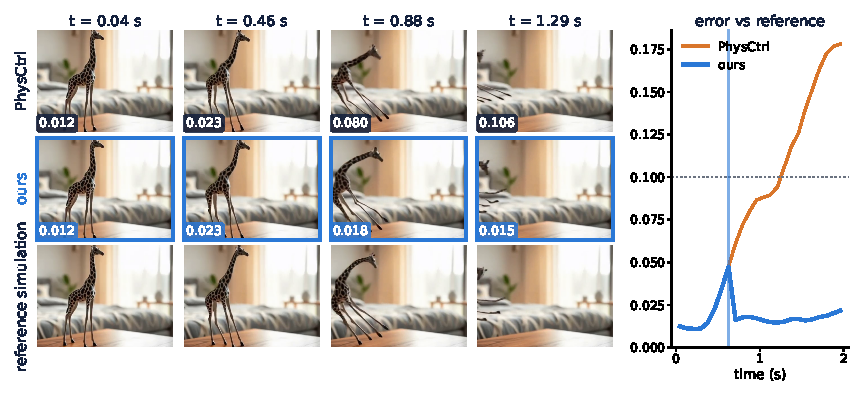
\includegraphics[width=\linewidth]{fig/qual_video.pdf}
\caption{\textbf{Rendered video} of PhysCtrl's giraffe example with 3$\times$ its drag force, chosen by the rule fixed before rendering (median PhysCtrl error among rejected cases). Labels: per-frame error. Our check fails at frame 7 and the rest is re-simulated.}
\label{fig:qual-video}
% src: job 95 (Phase 9 pipeline); results/fig_qualitative/paper_video_selection.json
\end{figure}
PhysCtrl fails on contact because it ignores the collision: on the two rule-selected contact scenes its composed output nearly coincides with the two objects simulated apart (error 0.136 vs.\ 0.119, and 0.125 vs.\ 0.112), while ours follows the reference to 0.028 and 0.025 (\cref{fig:teaser}a; both scenes in the supplement).
% src: job 94 (paper_contact_*.npz)
On PhysCtrl's five image examples with 3$\times$ their drag force, our check rejected all five and the repair lowered the error 1.8--18$\times$ (from 0.061--0.222 to 0.013--0.034); with the forces as given, all five were accepted (\cref{fig:qual-video}).
% src: job 95, case_v2.json (blanket 0.089->0.031, chair 0.061->0.034, earphone 0.222->0.013, giraffe 0.086->0.018, penguin 0.073->0.030)
Shifted queries, both contact scenes and all ten videos are in the supplement.

\section{Limitations and conclusion}
\label{sec:conclusion}

\paragraph{Limitations.}
\emph{Scope.} We study elastic objects, PhysCtrl's base model and 2{,}048 points; at this resolution a simulator substep costs about the same on every grid we use, which a denser setting would change.
\emph{The reference.} Ground truth is PhysCtrl's own MPM simulator, the motion the generator imitates, not real-world motion; its contact between objects is the sticky contact of grid-based MPM, and it is not converged at our error scale for soft materials, drops and strong pushes (\cref{sec:res-reference}), so absolute risks there depend on the chosen time step.
\emph{Known regimes.} In a known regime a tuned setting is cheaper (0.13$\times$ in distribution, 0.50$\times$ on contact), and under shift M2 is as safe as ours within the reference's uncertainty at 0.29$\times$; our advantage is tracking the simulator when the regime is unknown, with a per-query decision.
% src: Phase 9 (always M1 in distribution, always M3 on contact); Phase 10c (M2)
\emph{Stiff materials.} Explicit simulation grows costlier with stiffness while generation does not, so generate-then-certify should pay most for stiff objects; but in exploratory tests at $E \ge 10^8$\,Pa the certificate, calibrated on softer materials, accepted 6 of 16 bad trajectories.
% src: pilots E1, E1b
\emph{Conservativeness.} The certificate rejects many good trajectories (it accepted 105 of 174 good ones in distribution and 1 of 45 on contact), which is where most of the remaining cost goes.
% src: results/p9_table (certificate counts)
\emph{Video-level evaluation.} We score 3D trajectories. A 7B open VLM judge with PhysCtrl's prompt could not tell reference videos from PhysCtrl's (supplement).
\emph{Streams.} The amortised verifier is valid for stationary query streams only.

\paragraph{Conclusion.}
A fast learned motion prior is often wrong outside its training range or when objects collide, and neither the prior nor a simulator setting tuned on familiar queries says when.
Spending a few short simulator windows on each generated trajectory turns that silence into a calibrated accept-or-reject decision, and re-simulating only the uncertified suffix, from a cheap shadow's state and with the switch to a contact-resolving setting timed by that shadow, keeps the cost below simulating every query.
In pre-registered tests on fresh data, scored against three simulator time steps, only this pipeline stayed within a few points of simulating every query, in distribution, under shift and on contact, at less than its cost.
More broadly, a generative model need not be trusted or replaced wholesale: a little simulation, placed where its output is checked, can certify it.

{
    \small
    \bibliographystyle{ieeenat_fullname}
    \bibliography{main}
}
\end{document}
